在油气井冲砂洗井作业中，砂粒能否被携砂液有效携带出井筒是决定作业成败的关键。在水平井中，重力方向与砂粒运移方向垂直，因此不当的作业参数选择极易使砂粒在井筒内形成局部砂床。砂床的“锁定”效应易诱发工具和冲砂管柱砂卡，进而导致修井事故。

水平井筒内砂粒运移机理复杂，砂粒之间、砂粒与壁面间的相互作用强烈，传统的宏观模型难以精确描述低流速下砂床形成与动态演变过程。为此，学者们通过实验对砂砾运输的关键条件进行探究。Wick最早通过系统实验建立了临界携砂流速的量化方法[1]。King等人引入高粘度流体，揭示了粘度与临界流速的负相关关系[2]。李明忠团队提出了砂粒形状矫正系数，阐明井斜角对携砂效率的非线性影响，并指出井斜角在60°附近携砂最为困难[3-4]。王治中团队通过多参数实验，拟合出误差在±8\%以内的预测公式[5]。苏健鹏研究了不同砂粒直径与体积分数下的砂粒运动状态，分析了砂粒间流型转化机理，建立了砂粒运动流型相图，并系统分析了各因素对临界携砂流速的影响[6]。Danielson和Zeninali则分别从砂床压降关联和微细颗粒湍流运移角度深化了相关研究[7-8]。侯学文基于砂砾粒径、冲砂液排量、密度、粘度及现场实例井参数，建立了水平井冲砂洗井仿真模拟模型，分析了不同工况及作业因素对冲砂效果的影响[9]。Archibong-Eso等人以浆体流速、含砂体积分数为核心变量，探究二者及管道倾角对最小临界输送流速（MTC）与压力梯度的影响，评析了现有经验关联式的预测缺陷，并整合多组试验数据构建了带倾角修正的新型MTC关联式[10]。King等人通过比较不同粘度流体在倾斜管段内的冲砂效果，发现高粘度流体在倾斜管段内的携砂能力较弱[2]。Q.T. Doan等人针对疏松储层稠油水平井的出砂沉积问题，通过数值模拟阐释了原油粘度、流速、粒径对砂粒沉降与堆积的影响[11]。Najmi K通过开展不同流态下不同粘度流体的冲砂实验，发现流体处于湍流状态时，粘度增加会增强携砂能力；而处于层流状态时，结论则相反[12]。Piroozian A等人[13]和Sorgun M等人也指出[14]，层流状态下流体粘度升高会导致临界携砂速度上升，湍流状态下则导致其下降。然而，现有研究多聚焦于宏观临界携砂参数与预测，对砂床在冲砂过程中的动态行为关注不足，例如砂床的启动、砂丘迁移及形态转换等微观机理尚未明晰。

此外，在泥沙运动力学领域，相关成果丰硕。陈珊的室内试验揭示，散体沙的休止角随含水率升高呈递增趋势，但增长速率逐步减缓并最终趋于稳定，同时水流挟沙饱和度对动态休止角具有显著调控作用[15]。徐进超等人经研究表明，冲刷流量的增加会显著加速淤积厚度的削减，而水流流速的降低则会导致冲刷效率下降[16]。温庆文等人发现在固定床沙条件下输沙率与流量呈正相关关系[17]。周双运用高速摄像系统观测泥沙运动过程，通过实验与理论相结合的方法，深入分析了泥沙起动概率与推移质输移特性，并建立了适用于均匀与非均匀沙的输沙率计算模型[18]。段自豪发现非恒定流的速度偏度对泥沙运动具有显著影响，其输沙率普遍高于等效恒定流条件[19]。然而，这些成果基于开放水域与明渠流动，与井筒环空受限空间、高固相循环流动等实际工况存在显著差异，因此上述研究结论难以直接适用于井筒冲砂分析[20]。夏齐基于多相流实验平台及CFD-DEM数值模拟，分析了不同粘度流体在不同井斜角下的携砂效果[21]。洪贯洲采用计算流体力学-离散元法（CFD-DEM）全面描述了岩屑在井筒中的运移及沉积过程，并考虑流体、颗粒、钻杆以及壁面之间的相互作用[22]。朱娜进一步修正了大位移钻井两层动态岩屑运移模型，最终建立了起钻前岩屑床净化时间的求解方法[23]。Soepyan F B等人则对砂粒诸多运动状态所需的最小流速进行了定义[24]。

油气井现场作业表明，当井筒出砂严重时，修井管柱容易发生砂卡，特别是在水平井筒中。然而，当前研究对严重出砂的水平井在冲砂过程中砂床的动态行为和沉积机制认识不足，且缺乏适用于环空特殊构型的理论模型。为此，本研究拟通过室内物理模拟实验，系统探究冲砂液流速对底部砂床动态行为及水平井筒与冲砂管柱之间环空最终清砂效率的影响，旨在揭示环空内砂床的演变机理，并为油田现场冲砂作业的排量选择与优化提供理论依据与数据支持。

\section{水平井筒冲砂实验}
针对水平井冲砂洗井作业中，砂粒在与流向垂直的重力作用下极易在环空底部形成砂床，引发管柱砂卡事故。为揭示环空内砂床的动态演变机理，建立了水平井筒环空冲砂模拟实验装置，以清水和质量分数0.3\%的胍胶液为冲砂介质，系统研究了不同来流雷诺数下砂床前缘形态演化、自激振荡、分层运移及堆积高度变化规律。实验发现：清水冲砂过程中，随来流雷诺数的增加，砂床前缘依次经历拐点失稳、驻点形成与次生床分蘖等特征流态，并伴有周期性自激振荡现象；相比之下，胍胶液冲砂中砂床未出现振荡，前缘形态整体趋于流线型。两类流体在砂床顶部均表现为对流层与剪切滑移层的分层运移，但胍胶液组的滑移层厚度较清水组减小约45\%。基于量纲分析和实验数据，建立了砂头无量纲运移速度与局部雷诺数之间的关系。同时本文提出了一种砂床最大堆积高度的隐式预测方法，其验证误差小于1.15\%。结果表明，砂床堆积高度随进口雷诺数增加近似呈现线性递减，但砂头运移绝对速度慢，导致冲砂效率低。研究成果可为现场冲砂排量优选及砂卡风险定量评估提供理论依据

\subsection{实验装置及实验方法}
水平井筒环空冲砂模拟实验装置由可变流量泵送系统（含卧式离心泵和变频控制器）、流量计、供液桶、携砂液回收桶、亚克力透明管段（含内管、外管、导流锥、管撑）、高速观测相机和连接管路组成，实验装置如图\ref{fig:horizontal_washing_experiment_setup}所示。实验模拟$\phi 139.7$套管及$\phi 88.9$钻杆水平井环空自然冲砂工况，选取的实验管段外管内径为$Do=130\mathrm{mm}$，内管外径$Di=90\mathrm{mm}$，实验管段内壁光滑，有效工作长度约为$1.5\mathrm{m}$。

\begin{figure}[htbp]
	\centering
	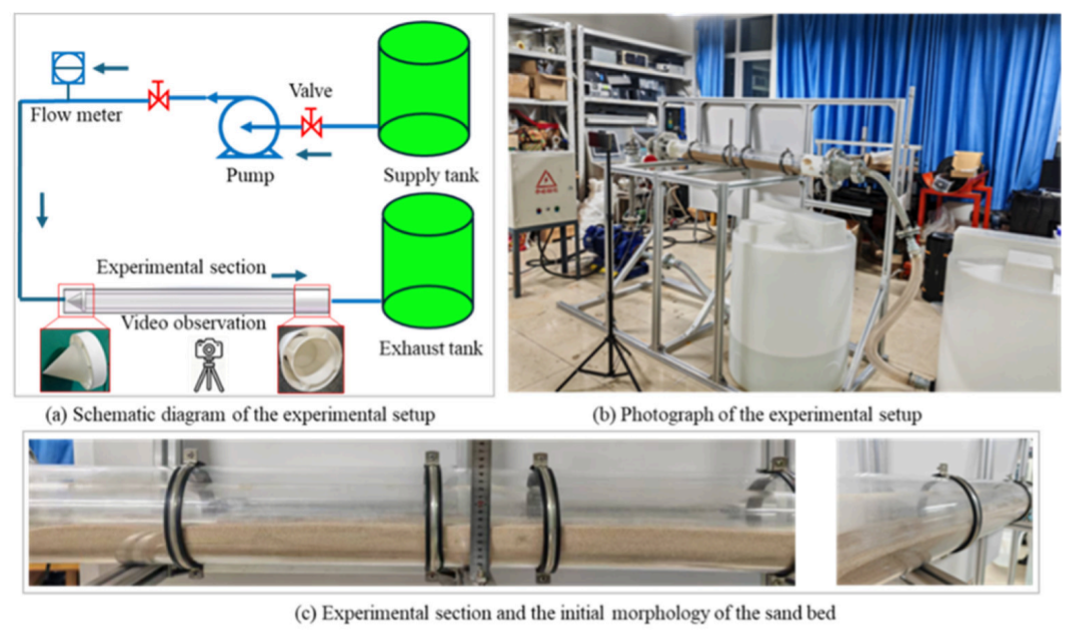
\includegraphics[width=0.9\textwidth]{figure/chapter2/horizontal-washing-experiment-setup.png}
	\caption{水平井筒环空冲砂模拟实验装置}
	\label{fig:horizontal_washing_experiment_setup}
\end{figure}



实验管段中，导流锥与管撑是确保环空流动稳定与几何精度的关键结构组件。导流锥安装于实验管段入口处，其前端锥形结构能够平顺引导流体，有效抑制入口复杂流态。导流锥后端的八个径向格栅是其整流结构的关键组成部分，不仅增强了内管的径向定位刚度，还将流体分割为多股均匀流束，有效促进动量分布均匀化，抑制大尺度涡旋的生成，从而确保进入实验段的流场在周向与径向上保持稳定、对称。此设计显著强化了整体的导流与均流效果，为实验提供了高度均匀的初始流场，抑制了流动的端面效应。管撑安装于实验管段出口端，具有结构定位与约束作用。管撑内缘与内管外壁配合，外缘与外管内壁固定。其主要作用是在出口端继续保持内外管的同心度，与入口端的导流锥形成两点定位，共同保证整个实验段环空间隙的沿程一致性。此外，管撑设计有轴肩，能够有效限制内管在流体作用或振动下可能产生的轴向窜动，防止实验过程中环空有效长度发生改变，从而保障实验边界条件的恒定。

实验开展前，将已知粒度组成的砂粒铺设于透明管段内部，确保砂床高度均匀一致，再像实验管段注入冲砂液。实验所用砂粒为标准石英砂，其参数如表\ref{tab:sand_params}所示。本文以清水和质量分数0.3\%的胍胶液（等效动力粘度12$\mathrm{mPa}\cdot \mathrm{s}$）作为冲砂液，对砂床运移行为进行分组研究。流量通过泵的运行频率调定，并确保每次实验中流速基本保持稳定。实验中，借助高速相机观测砂床的形态变化；此外，在相机的观测窗口设置一刻度尺（下文称其所在位置为“观测点”），利用该刻度尺定量测量砂床高度随时间的变化，以获取不同流量条件下砂床冲砂形态及运移的变化规律。实验的自变量为环空冲砂液平均流速，因变量为砂床的冲砂形态、运移速度和堆积高度等；实验中严格控制的常量包括环空几何结构、砂粒类型与初始质量、砂床初始铺设形态。

\begin{table}[htbp]
    \centering
    \caption{实验中使用的砂粒参数}
    \label{tab:sand_params}
    \begin{tabularx}{.9\textwidth}{XXc}
        \toprule % 顶部粗线
        参数 & 数值 & 单位 \\
        \midrule % 中间细线
        砾径中值 & 0.25 & mm \\
        砾径标准偏差 & 0.058 & mm \\
        砂砾密度 & 2500 & kg/m$^3$ \\
        砂砾堆积密度 & 1750 & kg/m$^3$ \\
        初始砂床高度 & 75 & mm \\
        \bottomrule % 底部粗线
    \end{tabularx}
\end{table}

\subsection{实验结果与讨论}
\subsubsection{清水冲砂}
水平井筒环空冲砂过程中，砂床的运移与沉积行为受多物理场耦合作用支配，涉及来流流量、流体物性、砂粒体积分数、流道几何约束等多个独立变量。若直接采用传统的数据拟合方法构建多变量经验关联式，不仅需要庞大的实验矩阵支撑，且所得公式往往量纲不一致、缺乏物理可解释性，难以推广至不同几何尺度或流体体系的工况。量纲分析法以Buckingham $\pi$定理为基础，能够将多变量物理问题转化为少数几个独立无量纲数群之间的函数关系，可有效约减变量空间，降低实验数据拟合的复杂度，且无量纲数具有明确的物理含义，不仅为从机理层面解释砂床行为的控制因素提供便利，也为实验结果在不同管径尺寸、不同流体体系的冲砂作业中推广奠定基础。鉴于本文实验涉及流量、粘度、砂床高度、运移速度、含砂体积分数等较高变量维度，且实验组数量受限于物理模拟条件，采用量纲分析法进行数据降维与函数关系建构，是实现从有限实验数据中提取普适性规律的合理且必要的技术路径。

在清水组实验中，名义值泵送流量$Q$为实验变量，并分别取$Q=8.5\mathrm{m^3/h}$、$11.8 \mathrm{m^3/h}$、$13.7 \mathrm{m^3/h}$、$15.4 \mathrm{m^3/h}$，用以探究来流情况对砂床运移行为的影响。胍胶液冲砂组旨在探究高粘度冲砂液对砂床运移行为的影响。对于管流，通常用流动雷诺数$Re$对流动性质进行综合表征，即
\begin{equation}
	Re=\frac{\rho U L}{\mu}
\end{equation}

式中，$\rho$和$\mu$分别为介质的密度和动力粘度；$U$为流动的特征速度。在计算泵为实验管段提供的来流雷诺数$Re_{in}$时，$\rho$和$\mu$根据冲砂液的物理属性取值；特征长度L取为环空的等效水力直径，即环空的内外径之差—$(D_o-D_i )$；特征速度U取为环空平均流速，根据流量$Q$和环空横截面积计算。再定义特征时间$T=(D_o-D_i)/U$，对于给定的时间$t$，可用$t^*=t/T$对其进行无量纲化处理。清水冲砂过程中来流雷诺数$Re_{\mathrm{in}}$随无量纲时间$t^*$的变化情况如图\ref{fig:incoming_Re_variation}所示，实验过程中供液桶水头持续降低等因素导致$Re_{\mathrm{in}}$呈现少量下降趋势，但相对变化量仅为2.83\%、1.72\%、0.81\%、1.31\%，因此，实验过程中的来流仍可视为定常。
\begin{figure}[htbp]
	\centering
	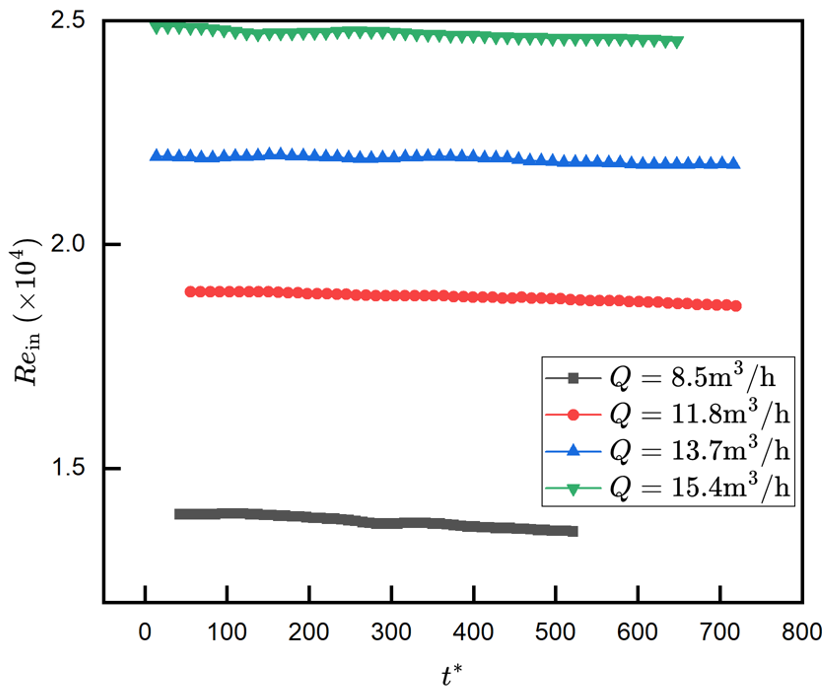
\includegraphics[width=0.7\textwidth]{figure/chapter2/IncomingReVStstar.png}
	\caption{进口雷诺数$Re_{in}$随无量纲时间$t^*$的变化情况}
	\label{fig:incoming_Re_variation}
\end{figure}

为定性描述砂床前缘的变化过程，本文利用拐点、驻点来刻画砂床前缘瞬时轮廓的特征，如图\ref{fig:stagnation_inflection_point}所示。设来流方向为y轴正方向，重力方向为x轴正方向。

\begin{figure}[htbp]
	\centering
	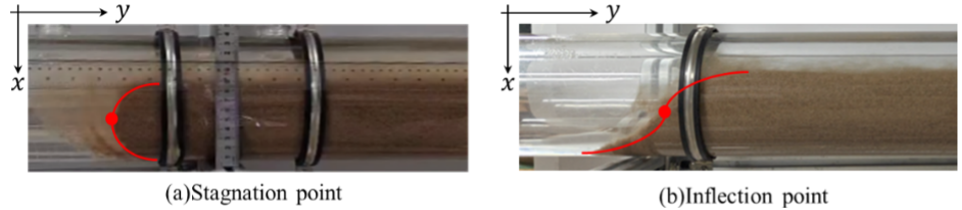
\includegraphics[width=0.7\textwidth]{figure/chapter2/stagenation-with-inflection-point.png}
	\caption{砂床前沿剖面中滞点与拐点的示意图（红色线条旨在示意性展示砂床前沿剖面形态，并不代表精确的定量测量结果）}
	\label{fig:stagnation_inflection_point}
\end{figure}

取来流雷诺数依次为$Re_\mathrm{in}=1.36×10^4 $、$1.89×10^4$ 、$2.20×10^4$三个实验组中砂床的形态变化作为研究对象。冲砂伊始，初始前缘上的砂粒在冲砂液冲击下出现短暂的剧烈翻滚，大量砂粒被扬起，弥散到冲砂液中形成高浓度砂团并随主流向后运移。当砂团经过砂床顶部时，携砂液中的部分砂粒因重力作用再次沉降，导致砂床出现不同程度的局部抬高现象，不同组别的前缘变化过程如图\ref{fig:bed_front_profile_Rein}所示。当砂床前缘呈现稳定状态时，冲砂进入准稳态阶段，但不同组别的前缘在这一阶段呈现出显著差异。

\begin{figure}[htbp]
	\centering
	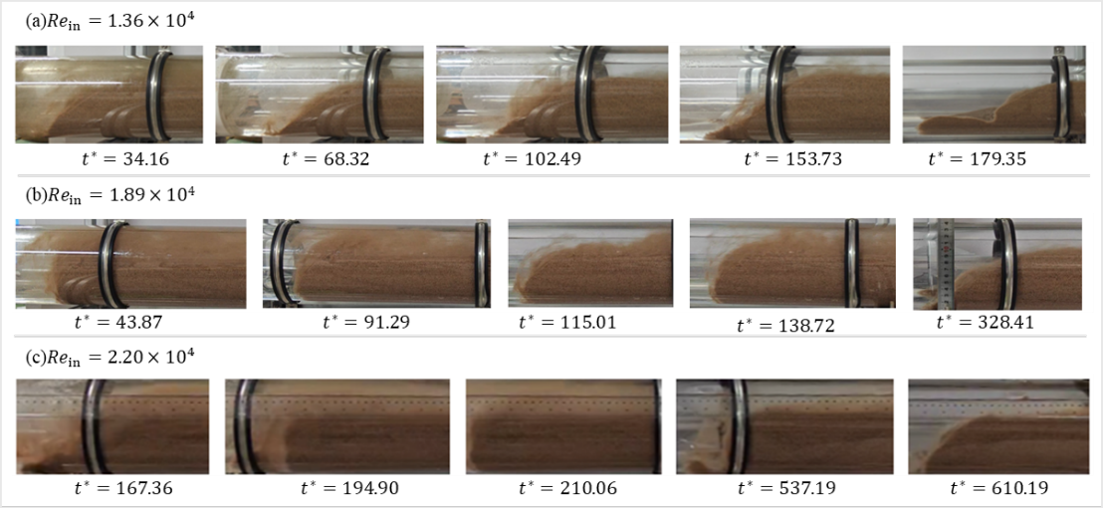
\includegraphics[width=0.7\textwidth]{figure/chapter2/bed-front-profile-VS-Rein.png}
	\caption{来流雷诺数对砂床前缘形态的影响}
	\label{fig:bed_front_profile_Rein}
\end{figure}

在$Re_{\mathrm{in}}=1.36×10^4$实验组（图\ref{fig:bed_front_profile_Rein}（a））中，当$t^*<153.73$时，随时间的推移，砂床前缘不断变瘦削，迎角不断减小。在$t^*=153.73$时，前缘轮廓线出现拐点并进一步产生失稳现象，分蘖成两个高度较小的次生床，这两个床层近似关于管道轴面两侧的平行平面对称分布。随时间的推移，次生床长度不断增大。次生床的形成主要由来流对砂床前缘的剪切应力分布不均所致，随着主床迎角的逐渐减小，拐点以下区域的来流剪切应力已不再整体高于砂粒运移阈值，这一临界条件的变化是次生床发育的关键诱因。$t^*>153.73$后，大量砂粒从主床前缘猝发性地卷入主流，在砂床上部形成高浓度携砂云团并随主流向后运移。同时，砂床前缘区域出现明显的边界层分离迹象，且环空顶部流体因流道收缩而流动加速。
在$Re_\mathrm{in}=1.89×10^4$实验组（图\ref{fig:bed_front_profile_Rein}（b））中，进入准稳态冲砂后，砂床前缘出现驻点。驻点以上区域的砂粒受流体剪切作用大量卷入主流，形成高浓度砂团；由于砂床前缘迎角较大，前缘与砂床顶面相交形成尖锐棱角，该几何特征直接诱发边界层分离，使得砂团以翻滚形态向下游运移。而驻点以下的砂粒，在来流的直接冲击下，甚至出现向左上方的逆向运移行为，随后受上部高速主流的阻滞作用逐渐减速，最终转向下游运移（$t^*=43.87$）。值得关注的是，驻点下方砂粒形成的砂团，在砂床上方的空间位置反而高于驻点上方砂粒形成的砂团，呈现出上下位置颠倒的独特现象。此外，砂粒运移呈现边运移边沉积的特征，且砂团与砂床前缘的运移速度均较$Re_\mathrm{in}=1.36×10^4$实验组有显著提升。随着时间的推移，砂床前缘轮廓线上的驻点持续向下迁移，在$t^*=91.29$时驻点消失在管壁上。砂床前缘的迎角随冲砂进行而持续减小。在$t^*=115.01$时，砂床前缘轮廓线出现拐点，在$t^*=328.41$时，进一步发育形成一个高度与长度均较小的次生床。
在$Re_\mathrm{in}=2.20×10^4$实验组（图\ref{fig:bed_front_profile_Rein}（c））中，进入准稳态冲砂后，砂床前缘在来流的冲蚀作用下，产生大量高浓度砂团，并迅速分蘖出次生床。随着冲砂的进行，主床前缘形成驻点，该实验组也出现了与图\ref{fig:bed_front_profile_Rein}（b）相似的砂床前缘上部高浓砂团和砂粒上下颠倒现象。在$t^*=167.39$时开始分蘖次生床，$t^*=194.90$时次生床与主床开始剥离。此后，在来流的冲蚀和来流冲击主床驻点下方砂床而形成的逆向扬起的共同作用下，次生床逐渐弥散在冲砂液中。在$t^*=537.19$时，在来流方向距主床一定距离处，开始出现完全剥离且前缘厚、中后部薄的次生小砂床。在来流流速近似恒定的情况下，前缘顺流区与逆流区共同作用处产生流速极低的空间，未及时运移的砂粒在此堆积，从而形成次生小砂床。


当携砂云团中的部分砂粒在砂床上方发生再沉积时，砂床高度随之抬升；与此同时，环空顶部的过流面积因砂床高度抬升而减小，流体在收缩流道内流动加速，强化了砂层运移，二者交替作用形成了独特的周期性动力振荡模式。图\ref{fig:bed_oscillation}为清水冲砂一个振荡周期内砂床运移的典型图示，砂团的形成和输运交替进行：第一个子图对应砂粒运移的镇静期，此时携砂云团或已沉降，或已运移至观测视野之外，砂床表面暂未出现大规模砂粒起动现象；第二个子图为携砂云团的生长期，大量砂粒从主床前缘被流体猝发式扬起，即将沿主流向后运移，主床前缘形态因砂粒起动而趋于模糊，但砂床顶部的轮廓仍保持清晰；第三个子图砂团在整个砂床表面呈现非均匀运移特征；第四个子图砂粒运移活动趋于停止，系统恢复至镇静状态。
\begin{figure}[htbp]
	\centering
	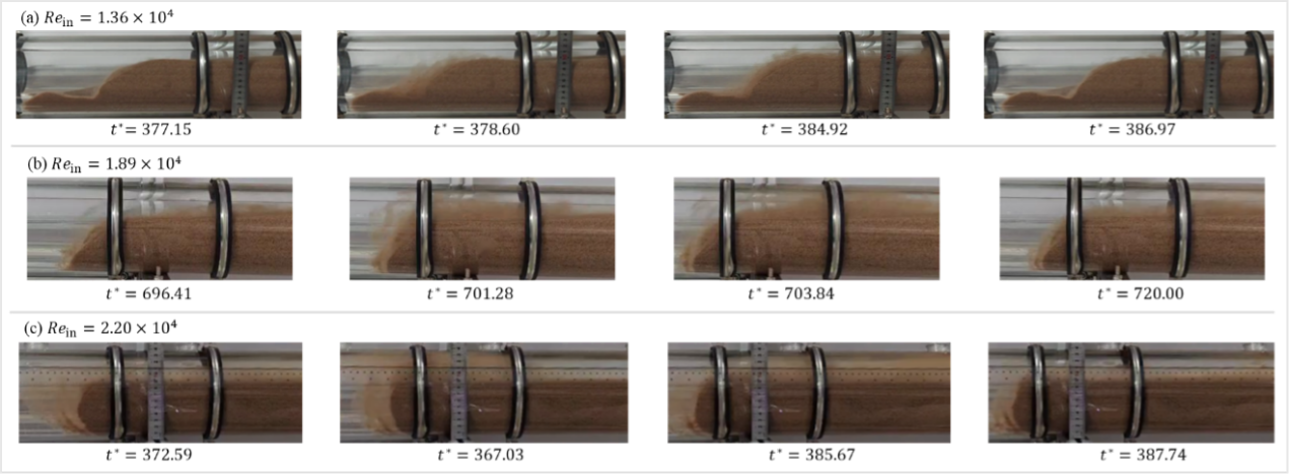
\includegraphics[width=0.7\textwidth]{figure/chapter2/bed-oscillation.png}
	\caption{清水冲砂中砂床运移的自激振荡现象}
	\label{fig:bed_oscillation}
\end{figure}

观测点处的砂床无量纲高度$h^*$随冲砂时间$t^*$的变化曲线呈现近“M”形，如图\ref{fig:M_shaped_bed_height}所示。以$Re_{\mathrm{in}}=1.36×10^4$组为例，在$t^*<200$时，砂床前端砂粒随主流向后运移，并在砂床顶部形成堆积，砂床高度明显升高。在$200<t^*<400$时，管壁的几何约束促使边界层实现再附着，观测点处流体不仅流速较高，还存在较大的向下速度分量，进而对砂床顶部施加显著的剪切应力，加速砂粒的侵蚀与流失，使得砂床高度呈现持续降低的演变趋势。在$400<t^*<500$时，砂床高度采样点的分布特征转为上凸形态，边界层分离点附近形成的逆压梯度，导致砂粒运移动能衰减并发生局部沉积。在运移的末期，即$t^*>500$时次生床长度持续拉长，主床前缘迎角已降至极小值，整体近似呈现流线型形态。
\begin{figure}[htbp]
	\centering
	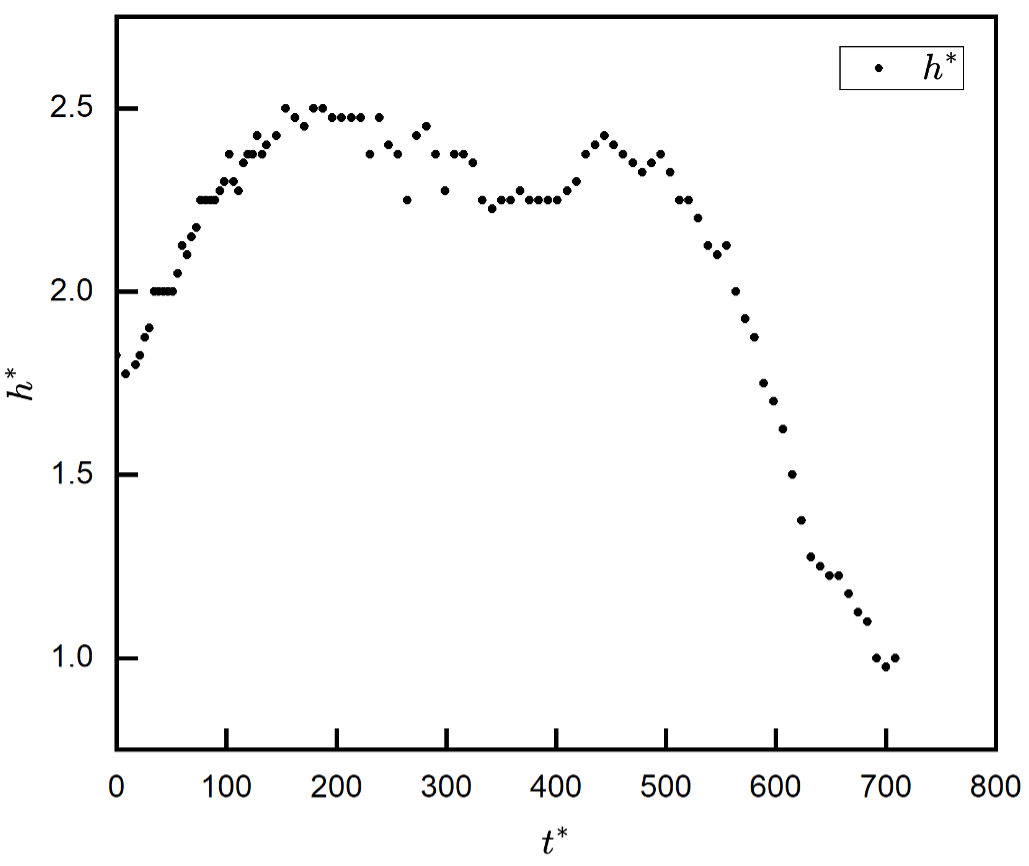
\includegraphics[width=0.7\textwidth]{figure/chapter2/M-shaped-bed-height.png}
	\caption{观测点处砂床高度随时间变化情况（$Re_{\mathrm{in}}=1.36×10^4$）}
	\label{fig:M_shaped_bed_height}
\end{figure}

砂床整体运移行为表明，由于砂粒尺寸细小且表面存在细微锐边，使得砂床堆积密实，同时与管道壁面形成显著的摩擦及锚定效应，进而产生较强的颗粒间内摩擦力与管壁摩擦力。砂床整体不发生迁移或滑移，以近似刚体状态与管道壁面保持相对静止。这一物理现象是绝大多数基于欧拉方法的数值模拟难以精准捕捉的，其核心原因在于砂粒初始堆积浓度过高，导致欧拉方法成立的前提假设难以满足，这也对新型模拟算法的开发提出了迫切需求。
\subsubsection{胍胶液冲砂}
胍胶液冲砂实验过程与清水冲砂相似，实验前调配一定浓度的胍胶增粘液，并在实验开始前使用粘度计测定其粘度。图\ref{fig:eta_gamma}中的流变测试结果表明：当剪切速率低于$720 \mathrm{s}^{-1}$时，胍胶液的表观粘度随剪切速率增加而降低，呈现出符合幂律模型[25]的典型剪切稀化现象。
\begin{equation}
	\eta=K\cdot \gamma^n
\end{equation}

\begin{figure}[htbp]
	\centering
	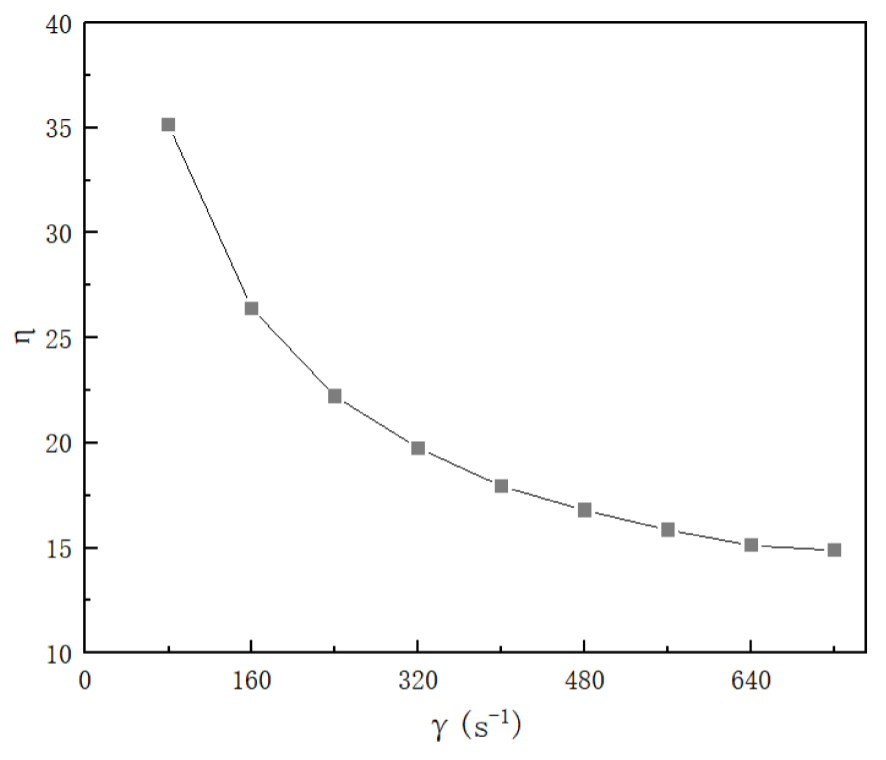
\includegraphics[width=0.7\textwidth]{figure/chapter2/eta-gamma.png}
	\caption{瓜尔胶的粘度-剪切速率关系}
	\label{fig:eta_gamma}
\end{figure}
将数据代入方程可得$\eta=22.53\cdot \gamma^{0.9764}$，对$80$–$720 \mathrm{s}^{-1}$范围内的数据进行了幂律拟合，其拟合优度$R^2=0.9946$。根据Metzner–Reed相关性，幂律流体流动的广义雷诺数可表示为

\begin{equation}
	Re_{\mathrm{MR}}=\frac{\rho V^{2-n} D^n}{K \left(\frac{3n+1}{4n}\right)^n\cdot 8^{n-1}}
\end{equation}

胍胶液的密度近似等于水的密度。将相关数据代入公式(2)后，可得出广义雷诺数约为 $Re_\mathrm{g}=2.048×10^3$，该值接近层流向湍流转变的临界值。

胍胶液冲砂组的来流雷诺数为$Re_\mathrm{g}=2.048×10^3$，处于弱湍流状态且携砂能力相对较弱，这与清水冲砂组情况有明显差异，图\ref{fig:bed_profile_guar_gel}为胍胶液组砂床前缘变化过程。$t^*<570.51$时，环空内仅在砂床前缘整形阶段产生了大范围高浓度砂团，随着冲砂的持续，砂床前缘不断瘦削并分蘖出次生床。$t^*=570.51$时，次生床运移速度追赶上主床，并与之融为一体。此后主床前缘迎角持续下降，冲砂液在砂床前缘携带砂粒向后呈现非均匀运移，在持续的冲砂作用下，砂床前缘逐渐平整，整个砂床轮廓趋于流线型。此阶段为冲砂的主要发生阶段，也是砂床前缘塑形的关键阶段。至$t^*=871.79$，砂床前缘及顶部轮廓已逐渐变为流线型，迎角持续降低，砂床形态变得更加瘦削，砂粒随主流向后呈均匀运移状态。至$t^*=1102.56$冲砂结束时，砂床整体呈现流线型。本组实验中并未出现明显的自激振荡现象。

\begin{figure}[htbp]
	\centering
	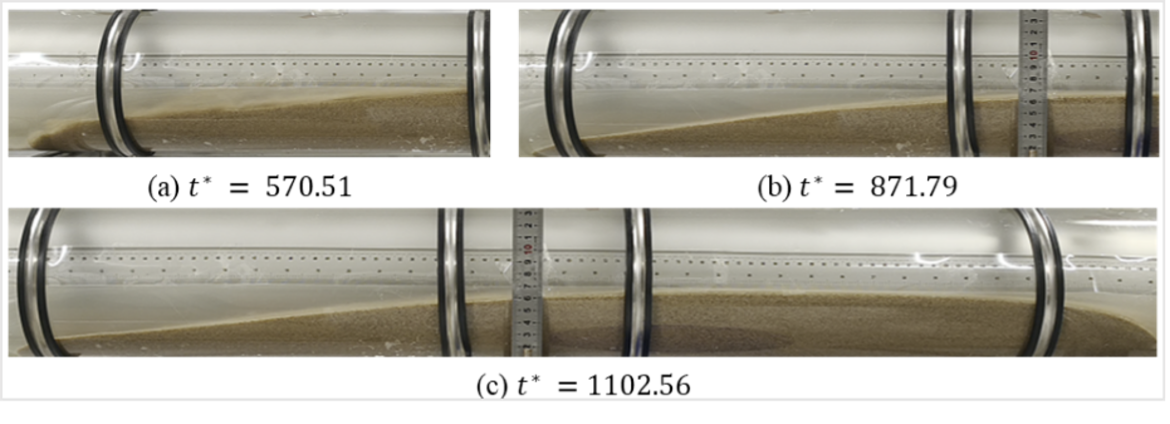
\includegraphics[width=0.7\textwidth]{figure/chapter2/bed-profile-guar-gel.png}
	\caption{观测点处砂床高度随时间变化情况（$Re_{\mathrm{in}}=1.36×10^4$）}
	\label{fig:bed_profile_guar_gel}
\end{figure}

在清水组和胍胶液组的准稳态运移阶段，砂床顶部的流动均表现出显著的分层运移行为，且这种分层特征在轴向远离前缘的区域尤为典型。具体可划分为两层：远离砂床顶部的流道是对流层，砂粒体积分数较低，分布范围较大，受主流拖拽作用显著，运移速度较快；靠近砂床顶部的是剪切滑移层，受床面剪切作用主导，砂粒体积分数较高，颗粒间相互作用强烈，运移速度较慢。测量剪切滑移层厚度发现，$Re_{\mathrm{in}}=1.36×10^4$组中厚度约为6.0mm，$Re_{\mathrm{in}}=1.89×10^4$组中约为6.2mm，$Re_{\mathrm{in}}=2.20×10^4$约为6.8mm，三组数值差异较小；相比之下，胍胶液组剪切滑移层厚度约为3.5mm，较清水组减小约45.0\%，表明在实验中清水对砂床的整体剪切作用高于胍胶液。

\subsubsection{砂床运移行为的控制因素分析及讨论}

本文基于室内实验观测现象与数据处理结果，构建表征砂粒运移行为特征的数学模型。实验数据解析以量纲分析为核心方法，从工程应用角度出发，砂粒运移速率与砂床堆积高度为冲砂洗井作业过程中的核心特征参数，因此将其作为后续数学模型的输出变量；模型输入变量则选取冲砂液粘度、密度及冲砂排量等工艺与水力关键参数。

本文假设在不同实验组中，沙床运移稳定后，砂头的速度$V_\mathrm{s}$与砂床堆积高度$h$基本不受砂床初始形态及初始高度的影响。砂头运移速度$V_\mathrm{s}$主要受控于来流流动条件，上文已用来流雷诺数$Re_{\mathrm{in}}$对其流动特征进行表征，$V_\mathrm{s}$对应的特征速度可取环空平均流速$U_\mathrm{in}$。相比之下，砂床堆积高度$h$的影响机制更为复杂，主要由砂床抬升所引发的流道堵塞效应主导，其演化受含砂液流的冲刷剪切作用与砂粒重力沉降作用共同耦合控制。在重力场恒定条件下，砂粒沉积效应主要与砂体积分数$\varphi_\mathrm{s}$及局部流速$U_\mathrm{l}$密切相关；而含砂液的剪切作用则取决于局部流速速$U_\mathrm{l}$、等效黏度$\mu_{\mathrm{eq}}$与等效密度$\rho_{\mathrm{eq}}$，可选取砂床顶部流道内的流动雷诺数$Re_\mathrm{l}$作为表征砂床堆积效应的综合评价指标。$Re_\mathrm{l}$与流体含砂量密切相关，根据流动连续性方程，流道中砂体积分数$\varphi_\mathrm{s}$与砂头运移速度$V_s$存在内在关联；同时，砂床抬升所引发的堵塞效应并非局部现象，也受砂床运移速度$V_\mathrm{s}$的制约。因此，在构建砂床高度的数学模型时，应充分纳入砂头运移速度$V_\mathrm{s}$的影响。综合上述，需要找到以下两个关系

\begin{equation}
    \begin{cases}
        V_s^* = V_s^*(Re_{\mathrm{in}}) \\
        Re_1 = Re_1(Re_{\mathrm{in}})
    \end{cases}
\end{equation}

实验中定量测得的砂头位置随时间的变化关系如图\ref{fig:p_star_VS_t_star}所示，图中以来流流量$Q$为参数。图中砂头的无量纲位置$p^*$是用砂头的实际位置与内外管径之差($D_o-D_i $)进行无量纲化后得到的；无量纲时间$t^*$是实际观测时间$t$用特征时间$T=(D_o-D_i)/U_in$进行无量纲化得到的。从图\ref{fig:p_star_VS_t_star}中可以看出，在准稳态运移阶段，$p^*$和$t^*$之间呈现线性变化规律。用线性函数对$p^* $($t^* $)进行拟合，可得砂头的无量纲运移速度$V_s^*$，图\ref{fig:Vs_star_VS_Rein}展示了$V_s^*$随$Re_{\mathrm{in}}$的变化情况，可见二者也近似呈现线性关系。用线性函数进行拟合得

\begin{figure}[htbp]
	\centering
	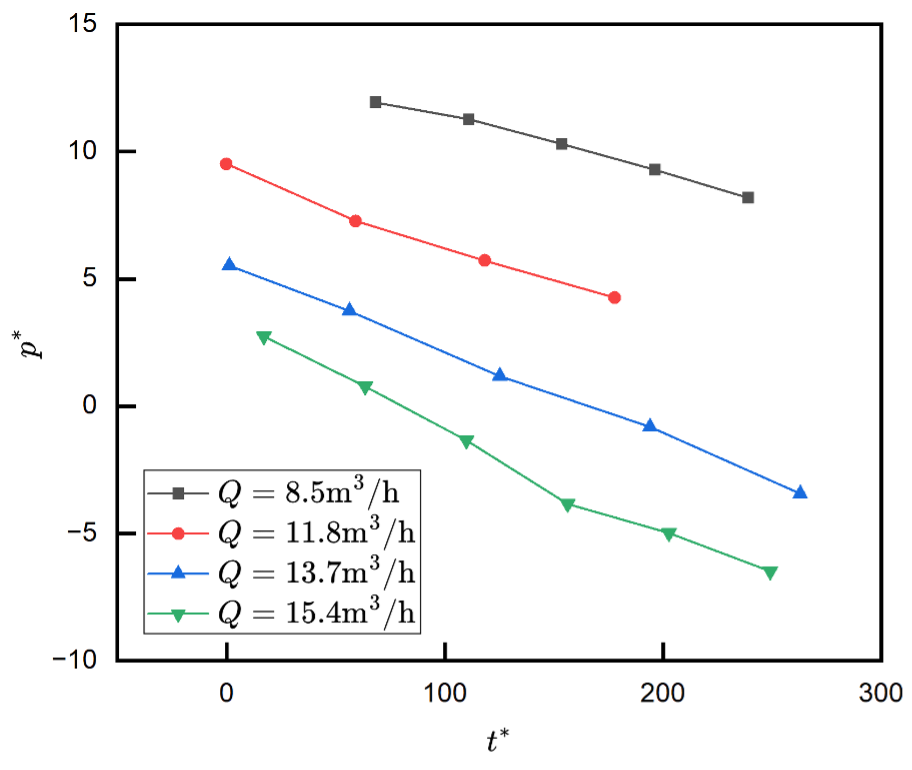
\includegraphics[width=0.7\textwidth]{figure/chapter2/p-star-VS-t-star.png}
	\caption{砂头位置$p^*$与冲砂时间$t^*$的变化关系}
	\label{fig:p_star_VS_t_star}
\end{figure}

\begin{figure}[htbp]
	\centering
	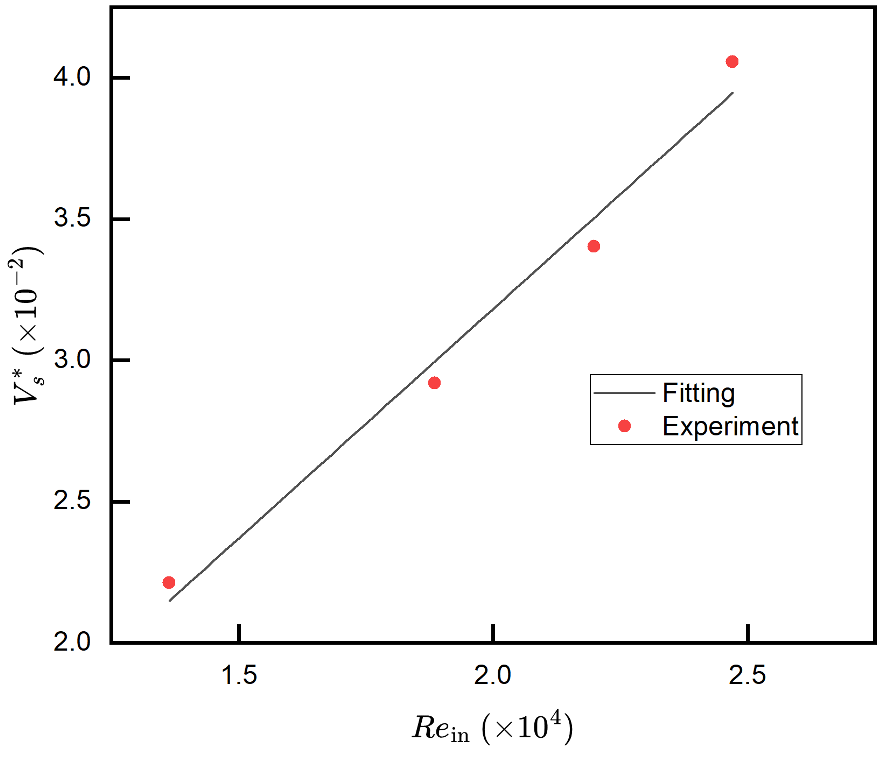
\includegraphics[width=0.7\textwidth]{figure/chapter2/Vs-star-VS-Rein.png}
	\caption{砂头运移速度$V_s^*$与进口雷诺数$Re_in$之间的关系}
	\label{fig:Vs_star_VS_Rein}
\end{figure}

\begin{equation}
	V_s^* = (1.62 \times 10^{-4} Re_{\text{in}} - 0.067) \times 10^{-2} \approx 1.62 \times 10^{-6} Re_{\text{in}}
\end{equation}

可见，$V_s^*$与$Re_{\mathrm{in}}$近似成正比例关系。

此外，实验中测量了由($D_o-D_i $)进行无量纲化无量纲最大高度$H^*$，其与$Re_\mathrm{in}$之间的变化关系如图\ref{fig:Rel_VS_Rein}所示；再根据流道几何计算局部雷诺数$Re_l$，其与$Re_\mathrm{in}$之间的变化关系如图\ref{fig:H_star_VS_Rein}所示。对于$Re_l$的计算，式（1）对应的当地参数取法为：$U$是砂床顶部通道中的平均流速，$ρ$是携砂液的平均密度，特征长度需选为流动通道的水力直径，计算表达式为$L=4S⁄P$，其中，$P$是润周，$S$是过流截面面积。根据实验中观测的现象，可做合理假设：砂床的上顶面是水平面，可结合砂床的高度H和几何关系计算$P$。此外，洗井液含砂后会对等效密度和粘度产生显著影响，本文采用砂粒的体积分数$ϕ_s$作为基础参数定量表征洗井液含砂的影响，$\varphi_s$的计算可根据砂头的位移速度$V_s$、砂床的高度$H$和来流流量$Q$进行。由于流动通道中流速较快，实验中观测到流道中砂的浓度稀薄，含砂液与纯水的相对粘度$\mu_r$可按下式计算
\begin{equation}
	\mu_r= 1+2.5\phi _s
\end{equation}

\begin{figure}[htbp]
	\centering
	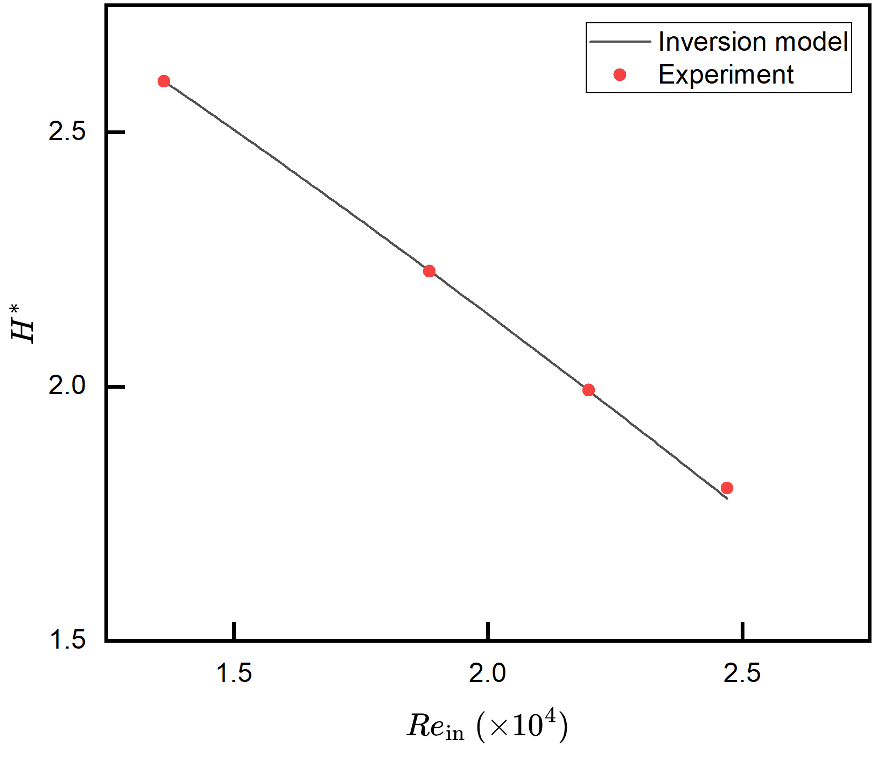
\includegraphics[width=0.7\textwidth]{figure/chapter2/H-star-VS-Rein.png}
	\caption{砂床最大高度$H^*$与来流雷诺数$Re_in$的关系}
	\label{fig:H_star_VS_Rein}
\end{figure}

\begin{figure}[htbp]
	\centering
	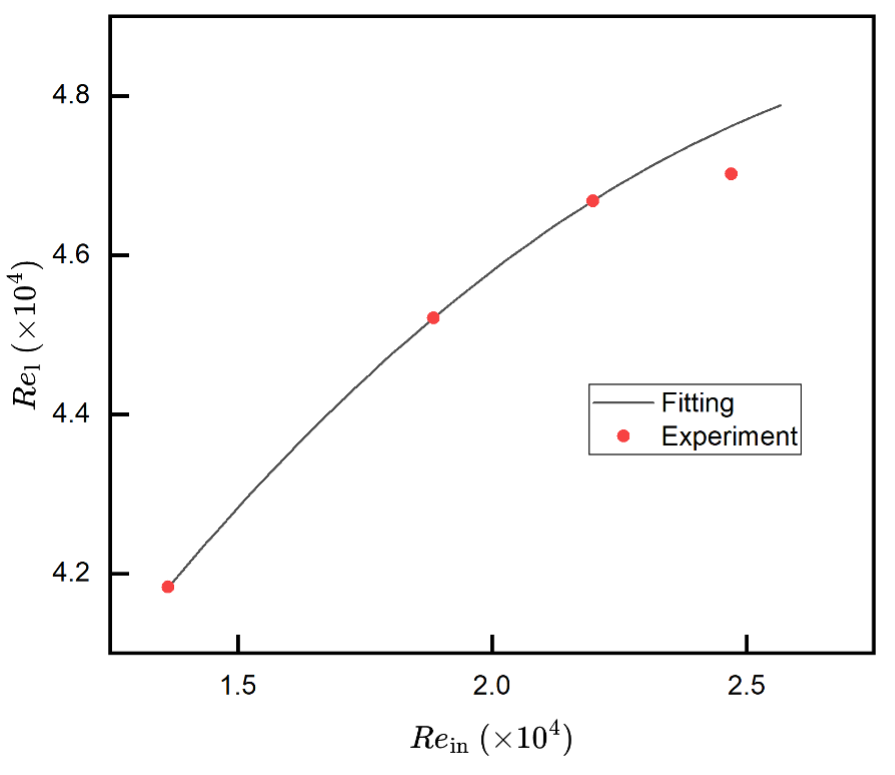
\includegraphics[width=0.7\textwidth]{figure/chapter2/Rel-VS-Rein.png}
	\caption{局部雷诺数$Re_l$与来流雷诺数$Re_\mathrm{in}$之间的关系}
	\label{fig:Rel_VS_Rein}
\end{figure}

$Re_l$和$Re_\mathrm{in}$之间的变化关系如图\ref{fig:Rel_VS_Rein}所示。随着$Re_\mathrm{in}$的增加，$Re_l$呈现单调递增的趋势。对前三组数据用二次函数进行拟合，第四组数据作为验证，可得
\begin{equation}
	Re_1 = -2.138 \times 10^{-5} Re_{\text{in}}^2 + 1.344 Re_{\text{in}} + 2.748 \times 10^4
\end{equation}
其中，第四组实验数据的相对误差为1.28\%，表明二次拟合模型在当前实验条件下充分捕捉了$Re_l$和$Re_\mathrm{in}$之间的关系。综上所述，方程(7)适用于来流雷诺数范围从$1.36×10^4$增至$2.47×10^4$且砂粒参数如表1所示的情况。

在实验数据的支撑下得到式(7)的关系后，可反解出$H^*$和$Re_{\mathrm{in}}$之间的关系。由于$H$和$S$在几何约束下呈非线性函数，所以$H^*$和$Re_in$是一个隐函数关系。本文通过数值方法求解得到了$H^*$的数值解，如图11所示，第四组实验中的$H^*$预测相对误差为$1.15\%$，预测精度较高。从拟合曲线的形状可以看出，$H^*$与$Re_{\mathrm{in}}$二者近似成线性关系，$V_s^*$产生显著变化时对$H^*$的影响较小，其主要原因是砂床的运移绝对速度低，局部流道中砂粒的体积分数较低，而砂粒的重力沉积作用相对较强。

从图\ref{fig:Vs_star_VS_Rein}中可以看出，砂头的无量纲运移速度较低，在4.0\%以下，表明水平段自然冲砂效率很低。砂床的消散动力主要依靠湍流来流的雷诺应力，其剪切分量导致了砂床表层砂粒的滑移及失稳，这种冲砂方法依赖于来流的脉动性；同时，砂粒间连接松散，雷诺应力中正应力分量的不均匀分布，会导致砂床结构破坏。后者在水平管道冲砂中占据主导地位，在这种冲砂机制下，砂头的形状会被重新塑造，迎角不断减小。在准稳态运移阶段，较小的砂头迎角限制了冲砂能力。若能有一种机制不断改变来流的冲砂方向，破坏锁死的条件，则有可能优化冲砂效率

虽然冲砂液扫除了砂头上游的分散砂粒，但在砂头后方产生了富集，导致砂床高度显著抬升，如图\ref{fig:H_star_VS_Rein}所示。如果在冲砂过程中拖动管柱，有可能导致管柱砂卡风险甚至比冲砂之前还要高。这种现象的主要原因是来流的速度方向和砂粒的重力沉积方向的差异，在水平井中这种沉积效应最为显著。如果在冲砂管柱上安装稳定器以改变流速方向，则有助于改善砂床在水平段的沉积。局部砂床的最大抬高高度随来流雷诺数线性递减，为减小管柱的砂卡风险，可采用增大泵送排量、使用高密度冲砂液等措施优化冲砂过程。

砂床顶部携砂液的雷诺数$Re_l$显著高于来流雷诺数$Re_{\mathrm{in}}$，这种效应主要是过流截面减小所致，而携砂液含砂量变化的影响较小。实际上，在所有实验组中，含砂率均处于较小范围（如图\ref{fig:phis_VS_Rein}所示），这意味着在更高的泵送排量下，局部通道中的流动湍动能越强，对砂床顶部的冲蚀能力和抵抗砂粒重力沉积的效应均越显著。若将实验结果向更高来流雷诺数进行外推，在砂床完全无抬高的极限情况下，局部雷诺数和来流雷诺数应为1:1的关系。考虑到图11中显示的砂床高度随来流雷诺数线性递减，节流形成的加速效应将迅速衰减。在更高的流量下，砂床的沉积效应将消失。可见，泵的排量对冲砂过程起到决定性作用。如果冲砂排量受限于设备的输出能力，也应按照实验结果，将砂床沉积高度控制在安全阈值以下。例如，工程中常将0.3倍以下的砂床高度视为安全，0.4倍以上视为高风险区。

\begin{figure}[htbp]
	\centering
	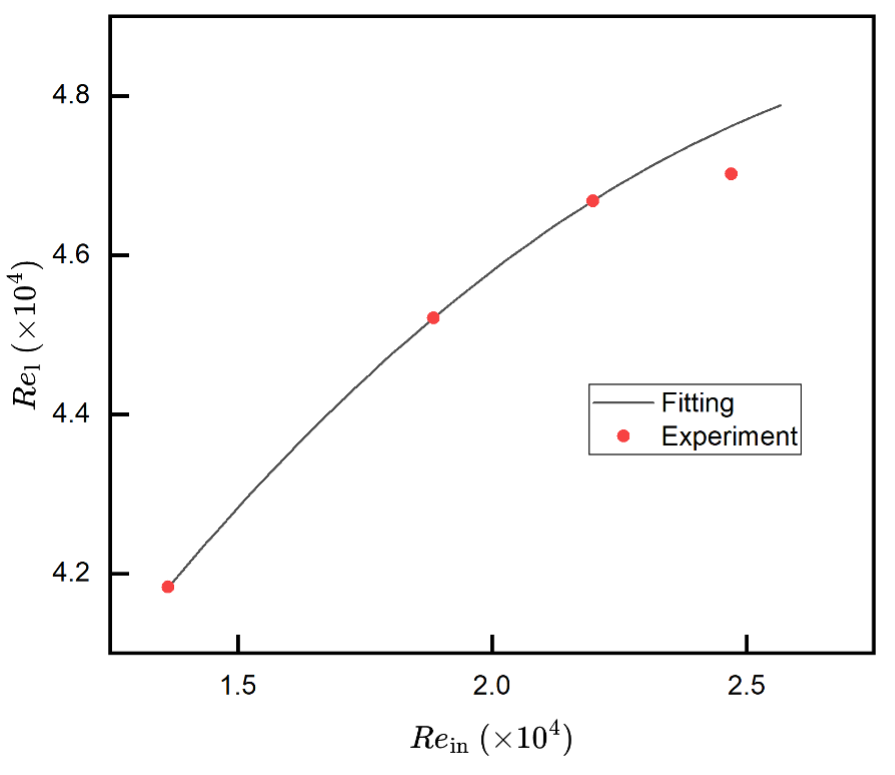
\includegraphics[width=0.7\textwidth]{figure/chapter2/Rel-VS-Rein.png}
	\caption{流道中含砂量$\phi_s$与$Re_{\mathrm{in}}$之间的反演关系}
	\label{fig:phis_VS_Rein}
\end{figure}


冲砂作业过程中，原本沿管柱相对分散分布的砂粒在局部管段出现高度聚集，而管柱及井下工具外表面存在的沟槽、台阶等结构特征进一步强化了砂粒滞留效应。在管柱拖动过程中，上述富集砂体极易引发工具遇卡，影响施工连续性。此外，在低流量冲砂条件下形成的次生砂床，以及高粘度冲砂条件下形成的流线型砂床，易在井下工具或管柱几何变径部位残留，形成连续或间断的沉积带，且这类沉积带难以被后续流体有效冲蚀运移，提高了现场施工作业的安全风险。此外，由于本文提出的物理模型是以无量纲数为研究对象的，其结果具有一定的普适性。该发现在工程中具有重要应用价值，对于水平井筒严重出砂的情况，可根据当地雷诺数估计砂床抬高后的高度，为拖动工具和管柱的砂卡风险定量评估提供依据。

夏齐[21]观察到，在水平井筒内的厚砂层表面颗粒在剪切力和冲击力作用下会通过跳跃和滚动方式向前迁移，这与本文的实验观测结果一致。然而当系统进入准稳态后，砂砾运移模式主要转变为以剪切滑动为主，以滚动运移为辅助。颗粒沉降导致的局部床层隆起现象进一步验证了洪贯洲[22]的CFD-DEM研究结论。将清水冲砂实验组对照发现：对于相同流体条件，湍流强度高，冲砂液携砂运输能力强砂床前缘运移速度快。此外，通过使用胍胶液进行冲砂实验发现，清水相较于胍胶液，具有更优异的冲砂性能。这一发现打破了“高粘度即高效”的传统观点，间接表明流体粘度与冲砂效率之间的关系并非简单的线性关系。本研究通过设置导流锥与管撑以消除环空偏心问题，即在理想同心环空条件下进行冲砂实验；未来将根据现场实际工况进行进一步实验，例如针对偏心工况下的洗砂效果开展深入研究。

本文基于自主设计的水平井筒环空冲砂模拟实验装置，以清水和质量分数0.3\%的胍胶液为冲砂介质，在不同来流流量工况下开展了室内环空冲砂物理模拟实验，系统观测了砂床前缘形态演化、自激振荡及分层运移等动态行为；在此基础上，采用量纲分析法，以来流雷诺数$Re_{\mathrm{in}}$为全局控制参数、局部雷诺数$Re_l$为桥梁变量，构建了砂头无量纲运移速度$V_s^*$与砂床最大堆积高度$H^*$的预测模型，得到以下主要结论：

（1）水平井筒环空内的冲砂过程具有显著的流速依赖性。清水冲砂条件下，随来流雷诺数$Re_in$从$1.36×10^4$增至$2.20×10^4$，砂床前缘依次经历拐点失稳、驻点形成、次生床分蘖与剥离等流态，并伴生由砂床抬升与流道收缩交替作用所引发的自激振荡现象；相比之下，胍胶液冲砂组（$Re_g=2.048×10^3$）处于弱湍流状态，携砂能力弱于清水组，前缘形态趋于流线型，未出现明显自激振荡现象。

（2）砂床顶部流动呈现显著分层特征，可划分为对流层与剪切滑移层。清水三组实验中，剪切滑移层厚度在6.0-6.8 mm之间，且随$Re_{\mathrm{in}}$增加而小幅增大；胍胶液组滑移层厚度约为3.5mm，较清水组减小约45.0\%，表明高粘度流体对床面的剪切作用更弱。

（3）砂头无量纲运移速度$V_s^*$处于极低水平（<4.0\%），表明水平段自然冲砂效率低下。$V_s^*$与$Re_in$呈良好正比例关系。砂床的最大无量纲堆积高度$H^*$随$Re_in$的增加近线性递减，其控制机制主要为流道收缩引发的局部加速效应，而含砂体积分数的影响较小。

（4）通过量纲分析构建了局部雷诺数$Re_l$与来流雷诺数$Re_in$的二次函数模型，验证误差为1.28\%，并可据此隐式求解砂床最大堆积高度$H^*$，预测误差为1.15\%，为工程中评估砂床抬高后的管柱砂卡风险提供了定量方法。

本研究从现象观测走向机理提炼，从定性描述走向定量表征，为严重出砂水平井的冲砂排量优选与砂卡风险评估提供了物理依据与分析工具。后续研究可在本文建立的方法框架上进一步拓展模型维度，发展高保真数值模拟与现场数据同化方法，最终形成从机理认知到工程决策的完整闭环，为复杂油气井修井作业的安全高效实施提供更为坚实的理论基础与技术支撑。

参考文献
1.	Wicks, M. Transport of Solids at Low Concentration in Horizontal Pipes. In Advances in Solid–Liquid Flow in Pipes and Its Application; 1971; pp. 101–124. 
2.	King, M.J.S.; Fairhurst, C.P.; and Hill, T.J. Solids Transport in Multiphase Flows—Application to High-Viscosity Systems. ASME. J. Energy Resour. Technol. 2001, 123, 200–204. 
3.	李明忠, 王卫阳, 何岩峰, 等. 垂直井筒携砂规律研究[J]. 石油大学学报: 自然科学版, 2000, 24(2): 4.
4.	李明忠, 王卫阳, 赵国景. 垂直井筒井液携砂流动规律研究及其在油井生产中的应用[J]. 实验力学, 2002(03): 385-392.
5.	王治中, 邓金根, 孙福街, 等. 井筒砂粒运移规律室内模拟实验研究[J]. 石油学报, 2006(04): 130-132+138.
6.	苏健鹏. 水平-竖直集气管道砂沉积规律与携砂特性研究[D]. 青岛: 中国石油大学(华东), 2019.
7.	Danielson, T.J. Danielson, Thomas J. Sand Transport Modeling in Multiphase Pipelines. In Proceedings of the Offshore Technology Conference, Houston, Texas, USA, 30 April-3 May 2007. 
8.	Zeinali, H. Effect of Near-Wall Turbulence on Selective Removal of Particles from Sand Beds Deposited in Pipelines. Ph.D. University of Alberta, Edmonton, Alberta, AB, Canada, 2012.
9.	侯学文. 水平井冲砂作业砂液两相流动与沉降特性研究[D]. 湖北: 长江大学, 2024.
10.	Archibong-Eso, A.; Aliyu, A.M.; Yan, W.; Okeke, N.E.; Baba, Y.D.; Fajemidupe, O.; Yeung, H. Experimental Study on Sand Transport Characteristics in Horizontal and Inclined Two-Phase Solid–Liquid Pipe Flow. J. Pipeline Syst. Eng. Pract. 2020, 11, 04019050.
11.	Doan, Q.T.; Doan, L.T.; Farouq Ali, S.M.; Oguztoreli, M. Sand Deposition inside a Horizontal Well—A Simulation Approach. J. Can. Pet. Technol. 2000, 39(10).
12.	Najmi, K. Particle Transport in Single-Phase and Multiphase Horizontal Pipes with Emphasis on the Effect of Viscosity; The University of Tulsa,Tulsa, Oklahoma, USA, 2015.
13.	Piroozian, A.; Ismail, I.; Yaacob, Z.; Babakhani, P; Ismail, A. Impact of Drilling Fluid Viscosity, Velocity and Hole Inclination on Cuttings Transport in Horizontal and Highly Deviated Wells. J. Pet. Explor. Prod. Technol 2. 2012 :149-456.
14.	Sorgun, M. Simple Correlations and Analysis of Cuttings Transport with Newtonian and Non-Newtonian Fluids in Horizontal and Deviated Wells. ASME. J. Energy Resour. Technol. September 2013, 135, 032903.
15.	陈珊. 变化水环境中散体沙休止角的初步研究[D]. 武汉: 武汉大学, 2014.
16.	徐进超, 李云, 宣国祥, 等. 船闸泄水作用下引航道中动水冲沙规律[J]. 水科学进展, 2016, 27(02): 186-195.
17.	温庆文. 紫坪铺水库清水下泄河道冲刷演变研究[D]. 雅安: 四川农业大学, 2022.
18.	周双. 推移质泥沙随机起动与输移机理研究[D]. 咸阳: 西北农林科技大学, 2022.
19.	段自豪, 陈杰, 蒋昌波, 等. 非恒定流作用下的推移质泥沙输移实验研究[J]. 中国科学：技术科学, 2019, 49(11): 1372-1382.
20.	Einstein, H.A. The Bed-Load Function for Sediment Transportation in Open Channel Flows; Tech. Bulletin No. 1026; US Department of Agriculture: Washington, D.C. USA, 1950.
21.	夏齐. 不同粘度液-砂流动规律及携砂性能研究[D]. 湖北: 长江大学, 2024.
22.	洪贯洲. 基于CFD-DEM方法对井筒内岩屑运移过程液固两相流动研究[D]. 黑龙江: 东北石油大学, 2024.
23.	朱娜. 大位移钻井岩屑运移规律与阻卡机理研究[D]. 北京: 中国石油大学(北京), 2022.
24.	Soepyan, F.B.; Cremaschi, S.; Sarica, C.; Subramani, H.J.; Kouba G.E. Solids Transport Models Comparison and Fine-Tuning for Horizontal, Low-Concentration Flow in Single-Phase Carrier Fluid. AIChE J. 2014, 60(1), 76–122.
25.	赵鉴楚,耿强.低聚物非牛顿流体流变参数的确定与流动计算[J].石油化工设计,2026,43(1):6-12+81.


\section{全井筒颗粒运移实验}

